\chapter{Methodology, Implementation and Results}


\section{Datasets Available on Networks, and Datasets Used}

\noindent {\bf SourceForge}

SourceForge is a web-based source code repository. It acts as a centralized location for software developers
to control and manage free and open source software development. It was the first to offer that service for
free to open source projects. The website runs a version of SourceForge Enterprise Edition, forked from the
last open-source version available. As of July 2011, the SourceForge repository hosts more than 300,000 projects
and has more than 2 million registered users, although not all are active.

\noindent {\bf Sourceforge.net}

SourceForge.net is the world’s largest Open Source software development web site, with the largest repository
of Open Source code and applications available on the Internet. Owned and operated by OSTG Inc. (``OSTG''),
SourceForge.net provides free services to Open Source developers. The SourceForge.net web site is database
driven and the supporting database includes historic and status statistics on over 100,000 projects and
over 1 million registered users’ activities at the project management web site. OSTG has shared certain
SourceForge.net data with the University of Notre Dame for the sole purpose of supporting academic and
scholarly research on the Free/Open Source Software phenomenon. OSTG has given Notre Dame permission to
in turn share this data with other academic researchers studying the Free/Open Source Software phenomenon.

\noindent {\bf Available Data}

SourceForge.net uses relational databases to store project management activity and statistics. There are over
100 relations (tables) in the monthly data dumps provided to Notre Dame. As of November 2005, the data warehouse was
almost 300 GB in size, and is growing at about 25 GB per month. Much of the data is duplicated among the monthly dumps,
but trends or changes in project activity and structure can be discovered by comparing data from the monthly dumps.
Queries across the monthly schema may be used to discover when changes took place, to estimate trends in project
activity and participation, or even that no activity, events or changes have taken place. To help researchers
determine what data is available, an ER-diagram and the definitions of tables and views in the data warehouse are provided.
For each month, the data warehouse includes three major parts:
\begin{itemize}
\item The tables supporting the SourceForge.net web site, for example, the tables user, group etc..
\item The tables used to store the statistics of the whole community, including daily page access, downloads etc.
\item The tables with the history information on the other tables.
\end{itemize}

\noindent {\bf Types of Data Used}

The following are the types of data that have been extracted from the SourceForge.net Research Data Archive for
the use in our project:
\begin{itemize}
\item Project sizes over time (number of developers as a function of time presented as a frequency distribution)
\item Development participation on projects (number of projects individual developers participate on presented as a frequency distribution)
\item Date of project creation (at SourceForge.net)
\item Date of first software release for a project
\item SourceForge.net ranking of projects at various times
\item Activity statistics on projects at various times
\item Number of projects in various software categories, e.g., games, communications, database, security, etc. Since all of the archived data is stored in a relational database, data to support FOSS investigations will be extracted using SQL queries against the data warehouse.
\end{itemize}
The first two items mentioned were used to create a ``collaboration social-network”, and also
to discover scale-free distributions among developer activity and project activity.

\section{Methods and Techniques}

\subsection{Weight Assignment}

\noindent {\bf Problem statement:}
Assign weights to an unweighted network dataset to obtain a clear and complete view of the network.

\noindent {\bf Dataset Used:}
\begin{enumerate}
\item {\em Co-authorship data}: This dataset contains authors where they are represented by the unique author's ID's.
A relation exist between two author ID's only if both have coauthored a book. Each author can be involved
in writing more than one book. In the graph format authors are represented by nodes or vertices and the
relations between them are represented by the presence of edge between them.
This is an undirected graph having 757 vertices and 1000 edges. 

\item {\em Email Communication Data}: This dataset contains the IDs of individuals who are actively involved
in a communication network via email. A relation between two IDs exist if any one of the two individuals
communicate through email. In the graph format, individuals are represented by nodes or vertices and the
relations between them are represented by the presence of edge between them. This is a directed graph having 1133 vertices and 10903 edges.
\end{enumerate}

\noindent {\bf Pseudocode/Algorithm}

\noindent Data : Unweighted RawDataFrame\\
\noindent Result : Weighted data

\begin{itemize}
\item Step 1 : Convert the data frame into graphs . Directed or undirected based on the data.
\item Step 2 : Remove all self loops and repeated edges.
\item Step 3 : Compute the similarity score using the intrinsic graph attributes.
\item Step 4 : Determine the weights from the similarity score.
\item Step 5 : Assign weights to each edge of the graph.
\item Step 6 : Generate weighted data file.
\end{itemize}

\noindent {\bf Procedure}

Given an unweighted social network dataset, it is possible to convert it into a weighted datagraph by
considering the features which are intrinsic to the graph. This process is performed using R software
which is a data mining tool for Big data as described previously. Further, R packages such as igraph,
sna, linkcomm and network, which again have been mentioned earlier, are used. Initially, a feature-rich
social network data is collected. It is converted into graphs. Outliers like self loops and repeated edges
are removed. A similarity score is calculated from a formula devised by taking into account the network
attributes and their definitions depending upon the data. Weights are computed from the score and are
assigned to each edge of the graph. Finally, these weights are appended to the input data and a new weighted dataset file is created.  

%\pagebreak
\noindent {\bf Results}

Results of the analysis are shown in Tables 4.1 and 4.2.

\begin{table}
\centering
\begin{tabular}{rr}\\ \hline
\multicolumn{2}{c}{Input}\\ \hline
FromNodeId &     ToNodeId\\ \hline
84424   & 276  \\
84424   & 1662 \\
84424   & 5089 \\
84424	& 6058 \\
84424	& 6229 \\
84424	& 10639 \\
84424	& 16442 \\
84424	& 19325 \\
84424	& 19834 \\
84424	& 20113 \\
84424	& 21937 \\
\vdots  & \vdots \\ \hline
\end{tabular}\\
\begin{tabular}{rrr}\\ \hline
\multicolumn{3}{c}{Output}\\ \hline
FromNodeId &     ToNodeId & Weight\\ \hline
84424   & 276  & 0.1549\\
84424   & 1662 & 0.1549\\
84424   & 5089 & 0.1549\\
84424   & 6058 & 0.1549\\
84424   & 6229 & 0.1549\\
84424   & 10639 & 0.0684\\
84424   & 16442 & 0.0684\\
84424   & 19325 & 0.0684\\
84424   & 19834 & 0.0684\\
84424   & 20113 & 0.0684\\
84424   & 21937 & 0.0684\\
\vdots  & \vdots & \vdots\\ \hline
\end{tabular}\\
\caption{Co-authorship Data}
\end{table}


\begin{table}
\centering
\begin{tabular}{rr}\\ \hline
\multicolumn{2}{c}{Input}\\ \hline
FromNodeId &     ToNodeId \\ \hline
1          &  2  \\
1          &  3  \\
1          &  4  \\
1          &  5  \\
1          &  6  \\
1          &  7  \\
1          &  8  \\
1          &  9  \\
1          &  10  \\
1          &  11  \\
\vdots & \vdots \\ \hline
\end{tabular}\\
\begin{tabular}{rrr}\\ \hline
\multicolumn{3}{c}{Output}\\ \hline
FromNodeId &     ToNodeId & Weight\\ \hline
1          &  2  & 0.0928\\
1          &  3  & 0.1194\\
1          &  4  & 0.0911\\
1          &  5  & 0.0698\\
1          &  6  & 0.0893\\
1          &  7  & 0.0981\\
1          &  8  & 0.0663\\
1          &  9  & 0.0822\\
1          &  10  & 0.1088\\
1          &  11  & 0.0875\\
\vdots & \vdots & \vdots\\ \hline
\end{tabular}
\caption{Email Communication Data}
\end{table}

\pagebreak
\subsection{Sampling Based Influence Analysis for Large Networks}

\noindent {\bf Problem statement:} Given a network of a very large size conduct
influence analysis on it.

\noindent {\bf Dataset Used:}\\
{\em January 2009 SourceForge data}: This dataset contains developers where they are represented by the unique developer's ID's.
A relation exists between two developer ID's only if both have collaborated on a project. Each developer can be involved
in developing multiple projects. In the graph format developers are represented by nodes or vertices and the
relations between them are represented by the presence of edge between them.
This is a directed graph having 36111 vertices and 209491 edges.

\noindent {\bf Method}

The standard techniques for clustering fail when one applies them to very large
networks due to computational complexity. The alternative suggested here is to
identify the major subnetworks of such a large network first, and then to
conduct influence analysis for each of the large subnetworks. The question is
how one can identify the clusters within a network without a complete exploration
of the entire network. Here is where probabilistic methods help. Probability
theory, especially the Law of Large Numbers, says that under general conditions,
random sampling can be used to identify important features of a population.
Consider a large network to be a given population and apply random sampling
to extract a sample. Treat this as a randomly generated subnetwork. As long
as the sample size is reasonable, clustering algorithms will work efficiently
on the sampled subnetwork. Now apply the Law of Large Numbers and claim
that if the sampling is continued, then sooner or later, the nature of
clusters within the large network will emerge. Consequently, the influence
analysis conducted on a reasonable sized random subnetwork will closely
approximate the influence analysis of the entire network. One just needs
to continue sampling until the number of clusters obtained stabilizes.

\pagebreak
\noindent {\bf Pseudocode/Algorithm}

\noindent Data : Network Data\\
\noindent Result : Large Subnetworks, Influential nodes

\begin{itemize}
\item Step 1 :  Convert the network into a graph where $N$ is the total number of vertices,
directed or undirected based on the data.
\item Step 2 :  Initialize the sample size to $n$ = 10\% of $N$.
Sample a subnetwork consisting of $n$ vertices.
\item Step 3 : Apply the Fast Greedy clustering algorithm to the sampled subnetwork and
obtain the clusters therein. Drop all clusters of size less than 1\% of $n$.
\item Step 4 : Check whether the stopping rule (*) is satisfied. If yes, go to Step 6;
else go to Step 5.
\item Step 5 : Increment $n$ by 10\% (of $N$) and repeat Steps 2 and 3.
\item Step 6 : Complete the clustering of the entire network by assigning the unsampled
vertices to the identified clusters using the PageRank algorithm.
\item Step 7 : Perform influence analysis on each of the finally obtained clusters.
\end{itemize}
(*): The stopping rule used in this project is as follows: Let $a_i$ be the number of clusters
obtained in the $i$th iteration. Define $b_i = |a_{i+1}-a_i|$ and $c_i = |b_{i+1}-b_i|$. Stop
when $c_{i+1}\le c_i$.

\noindent {\bf Procedure}

Given a large social network dataset, it is possible to identify the influential individuals
by performing influence analysis on this network.
This approach is implemented using R software which is a statistical programming language.
R packages such as igraph, sna, network, ProNet and ergm are used. Initially, a feature-rich
social network data is collected. It is converted into graphs. Outliers like self loops and repeated edges
are removed. Subnetworks of increasingly large sample sizes are randomly extracted and
clustered. Once this stabilizes, the unsampled vertices are assigned to the obtained large
subnetworks using PageRank. Subsequently, influence analysis is performed on the identified clusters.

\noindent {\bf Results}

Results of the analysis are shown in Tables 4.3 and 4.4, and Figures 4.1 - 4.18.

\begin{table}
\centering
\begin{tabular}{rr}\\ \hline
\multicolumn{2}{c}{Input}\\ \hline
From & To\\ \hline
0 & 28234 \\
0 & 9031 \\
1 & 27082 \\
1 & 23805 \\
1 & 21702 \\
1 & 35191 \\
1 & 22520 \\
1 & 28220 \\
1 & 36 \\
\vdots & \vdots \\ \hline
\end{tabular}
\caption{January 2009 SourceForge Data}
\end{table}

\begin{table}
\centering
\begin{tabular}{rrr}\\ \hline
Sample percent & Number of vertices selected & Number of clusters found\\ \hline
10 & 3611 & 1\\
20 & 7222 & 5\\
30 & 10833 & 10\\
40 & 14444 & 10\\ \hline
\end{tabular}
\caption{Number of clusters versus sampling percentage}
\end{table}

\begin{figure}[htb]
\centering
\begin{minipage}{0.45\linewidth}
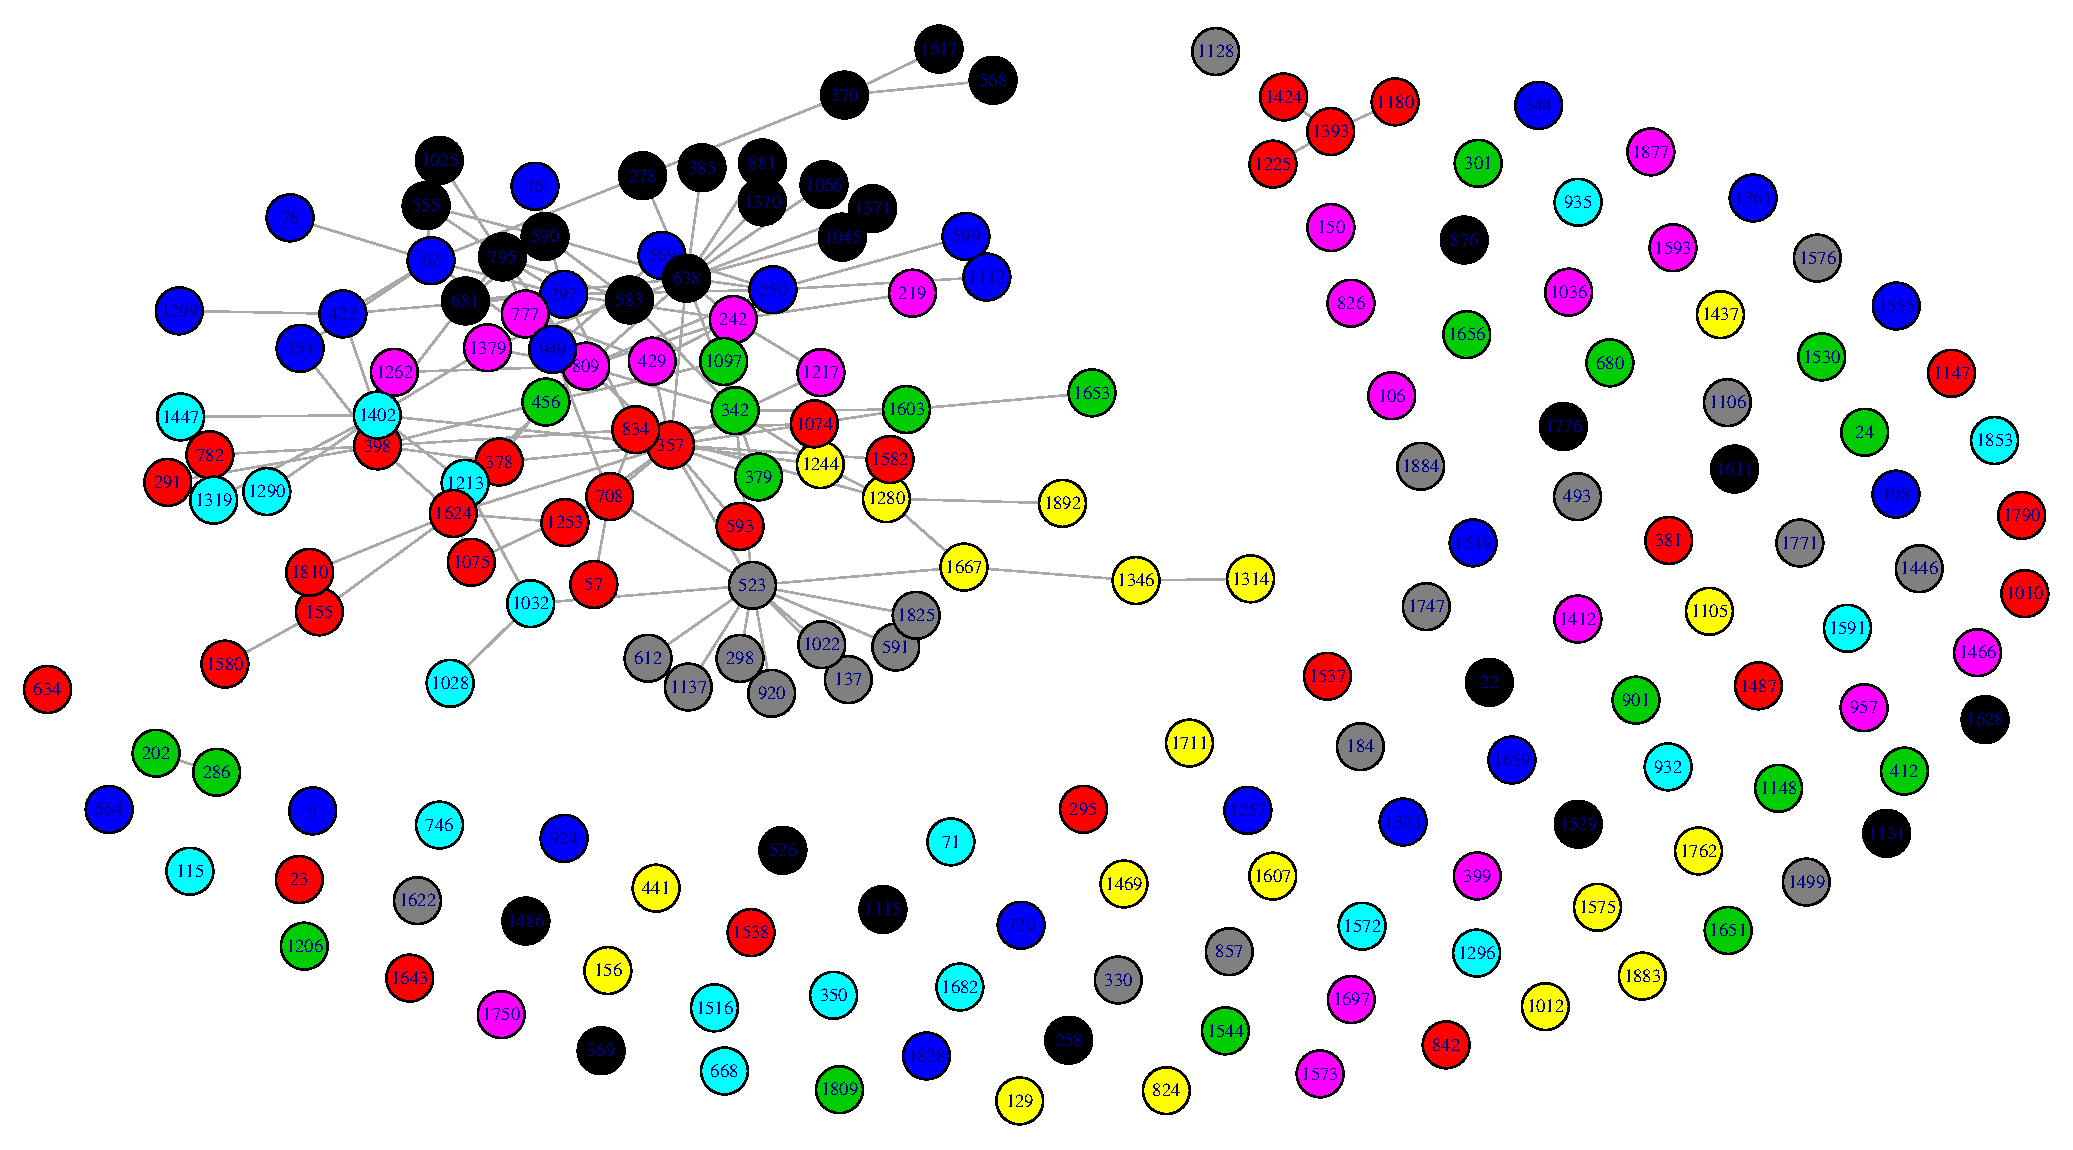
\includegraphics[scale=0.2]{Methods/10percent.eps}
\caption{Clusters with 10\% sampling}
\end{minipage}
\quad
\begin{minipage}{0.45\linewidth}
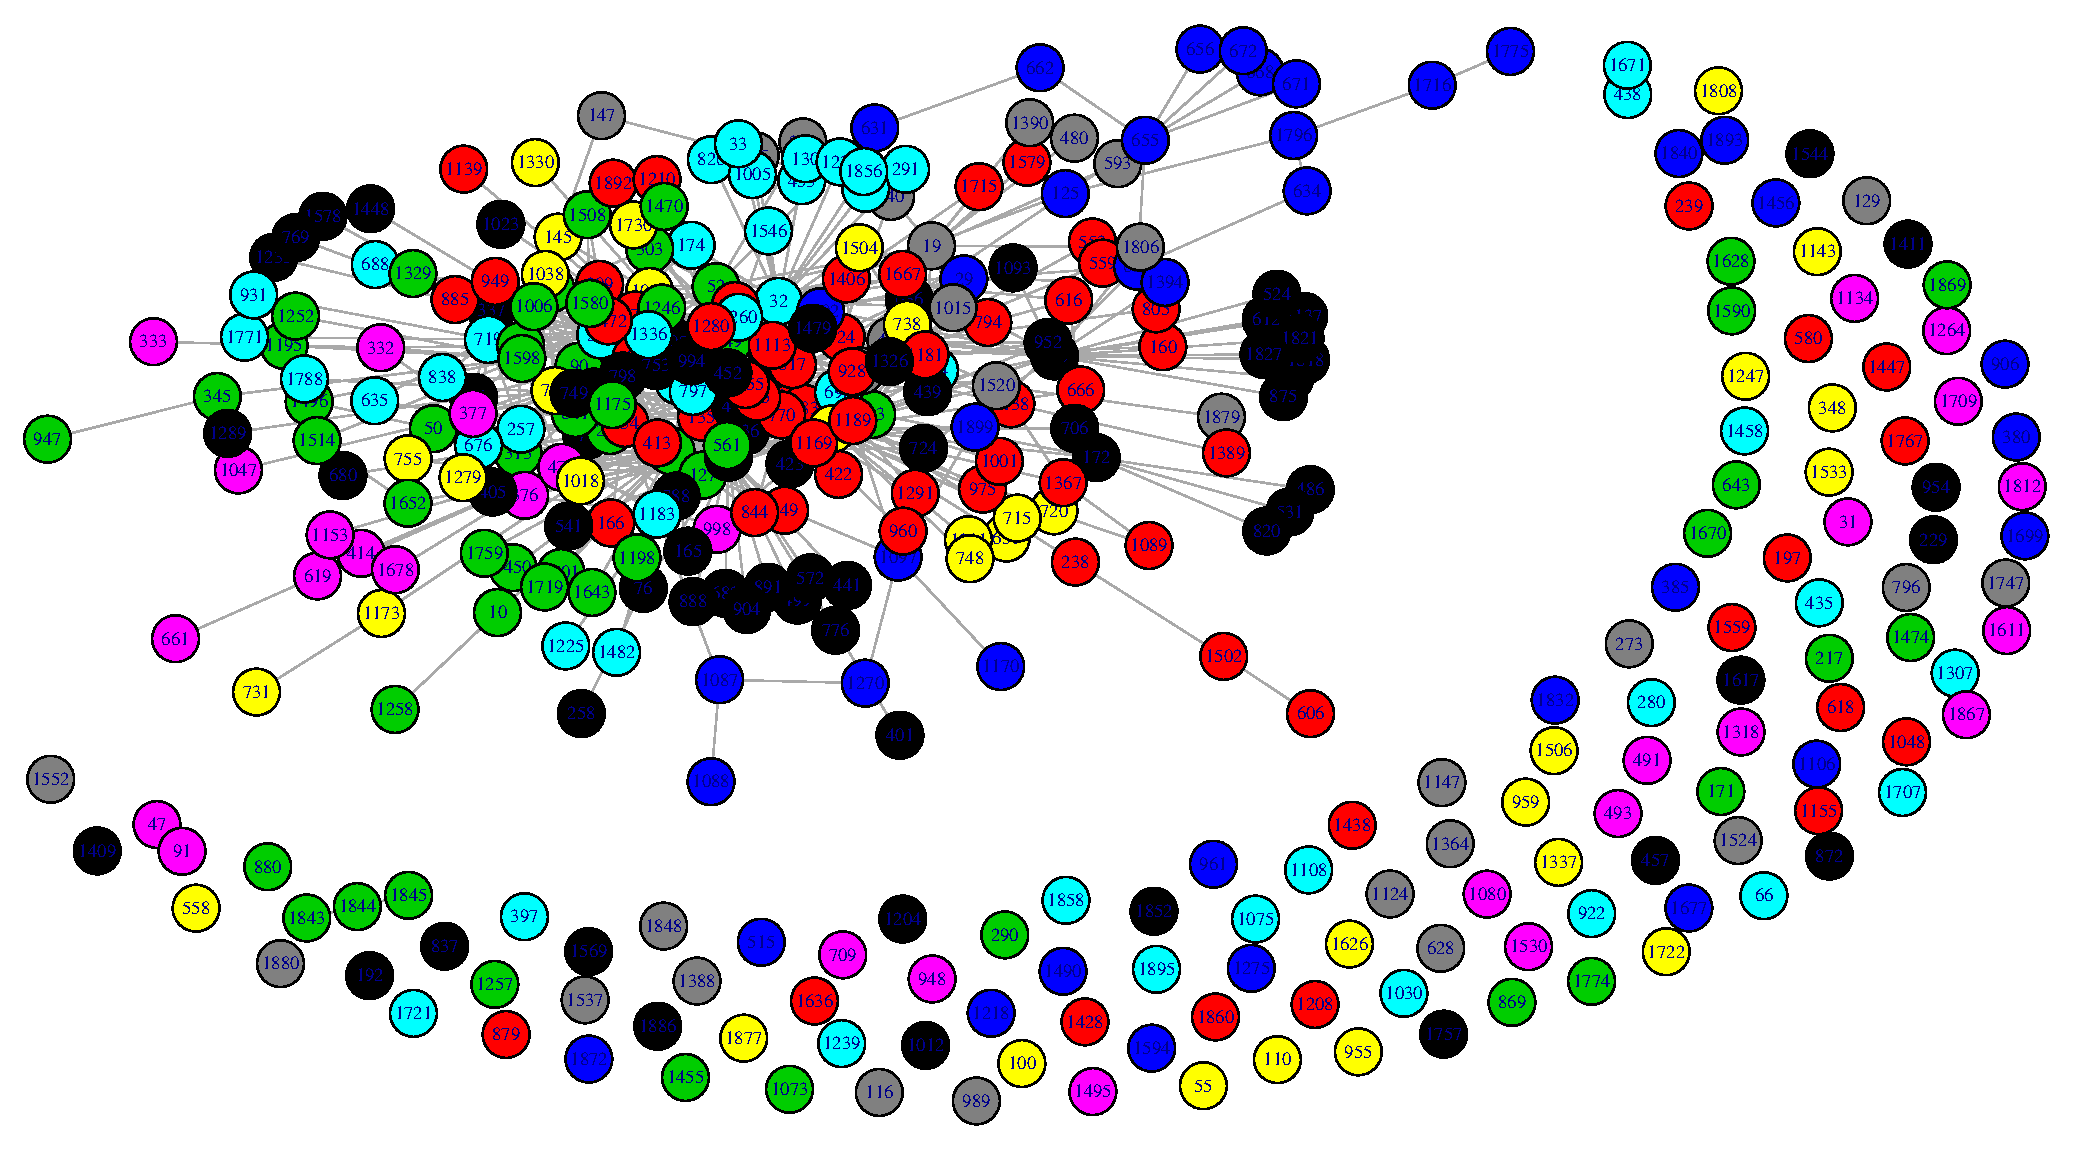
\includegraphics[scale=0.2]{Methods/20percent.eps}
\caption{Clusters with 20\% sampling}
\end{minipage}
\end{figure}
\pagebreak

\begin{figure}[htb]
\centering
\begin{minipage}{0.45\linewidth}
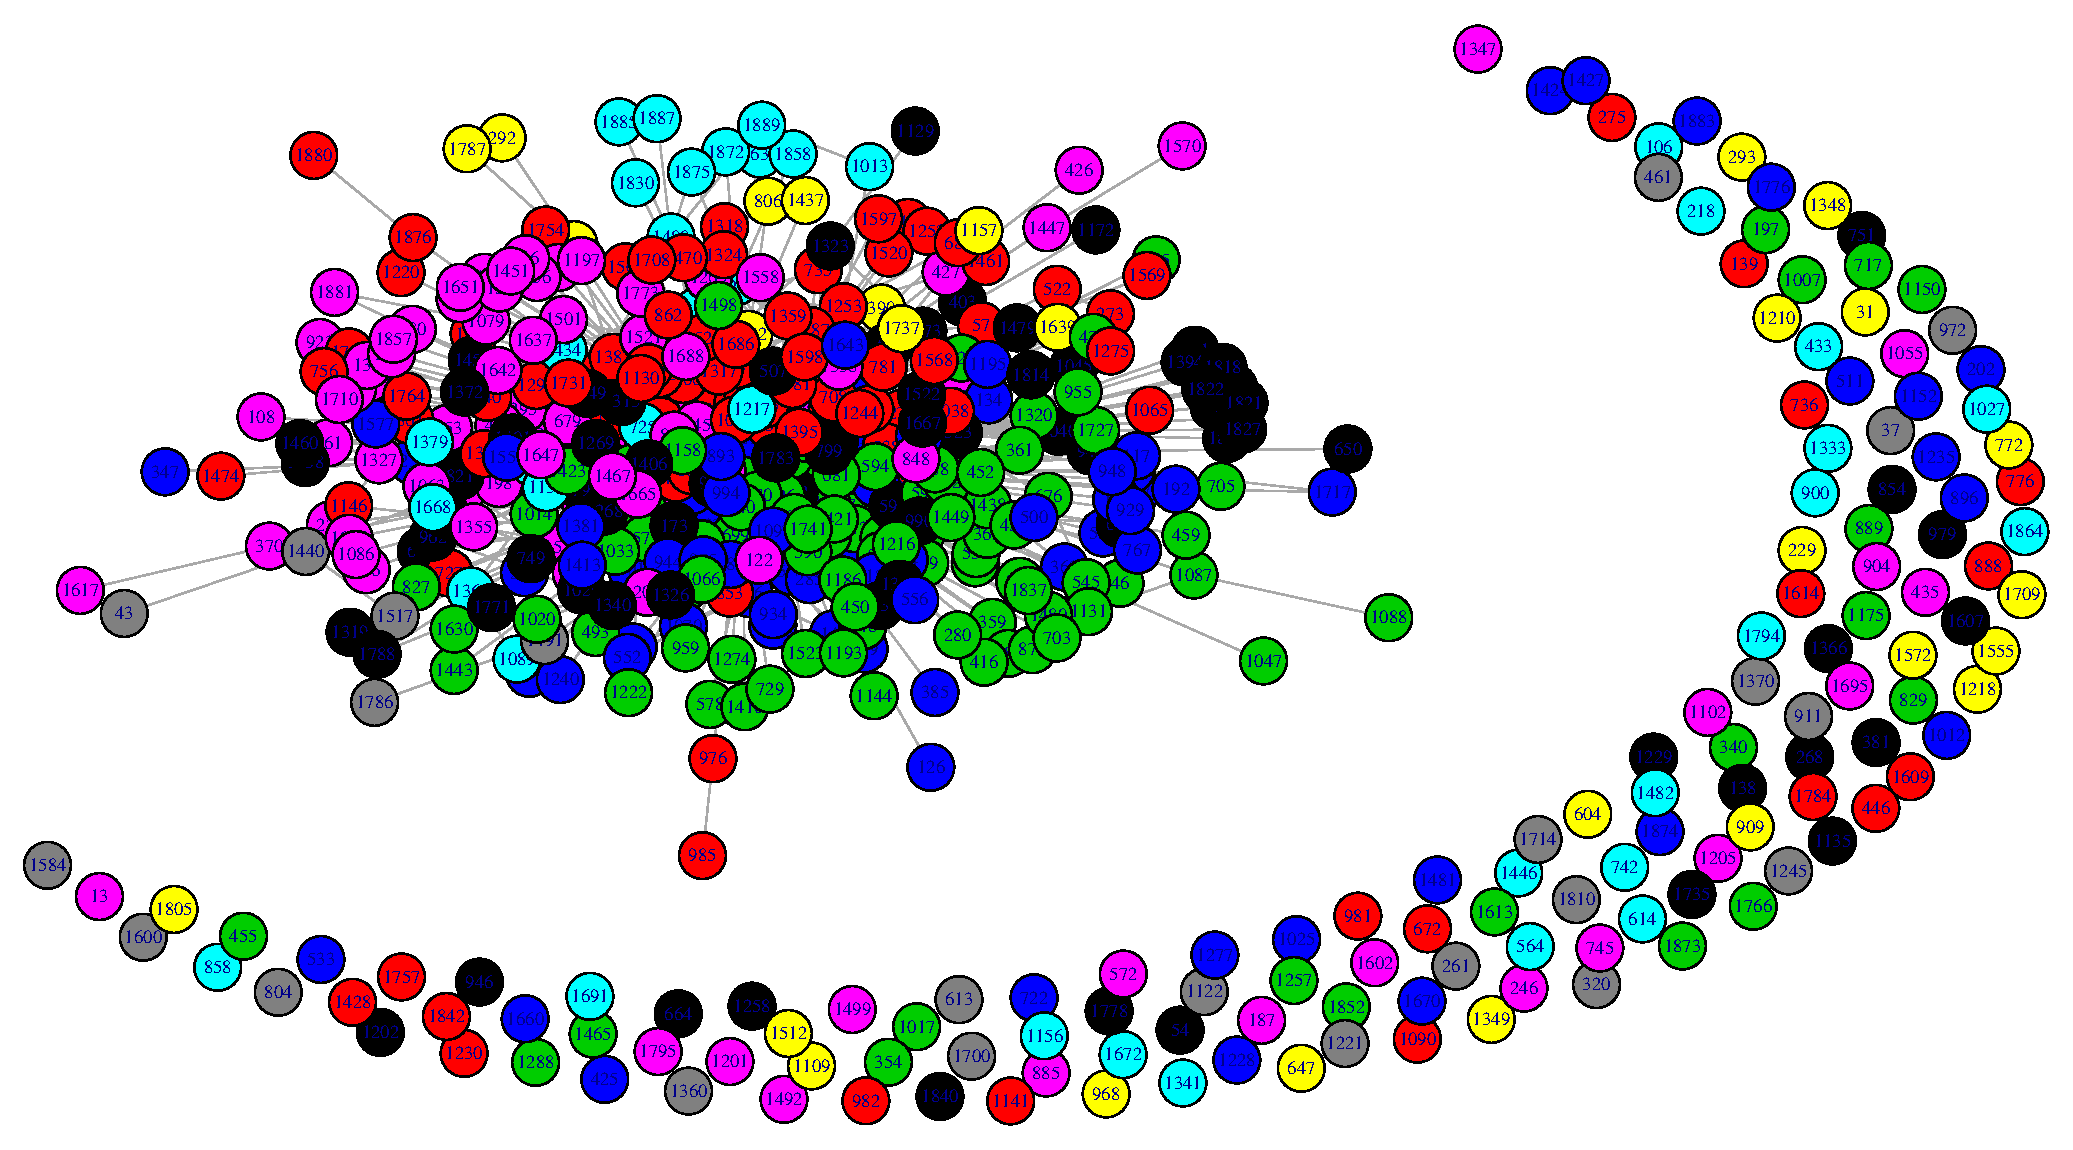
\includegraphics[scale=0.2]{Methods/30percent.eps}
\caption{Clusters with 30\% sampling}
\end{minipage}
\quad
\begin{minipage}{0.45\linewidth}
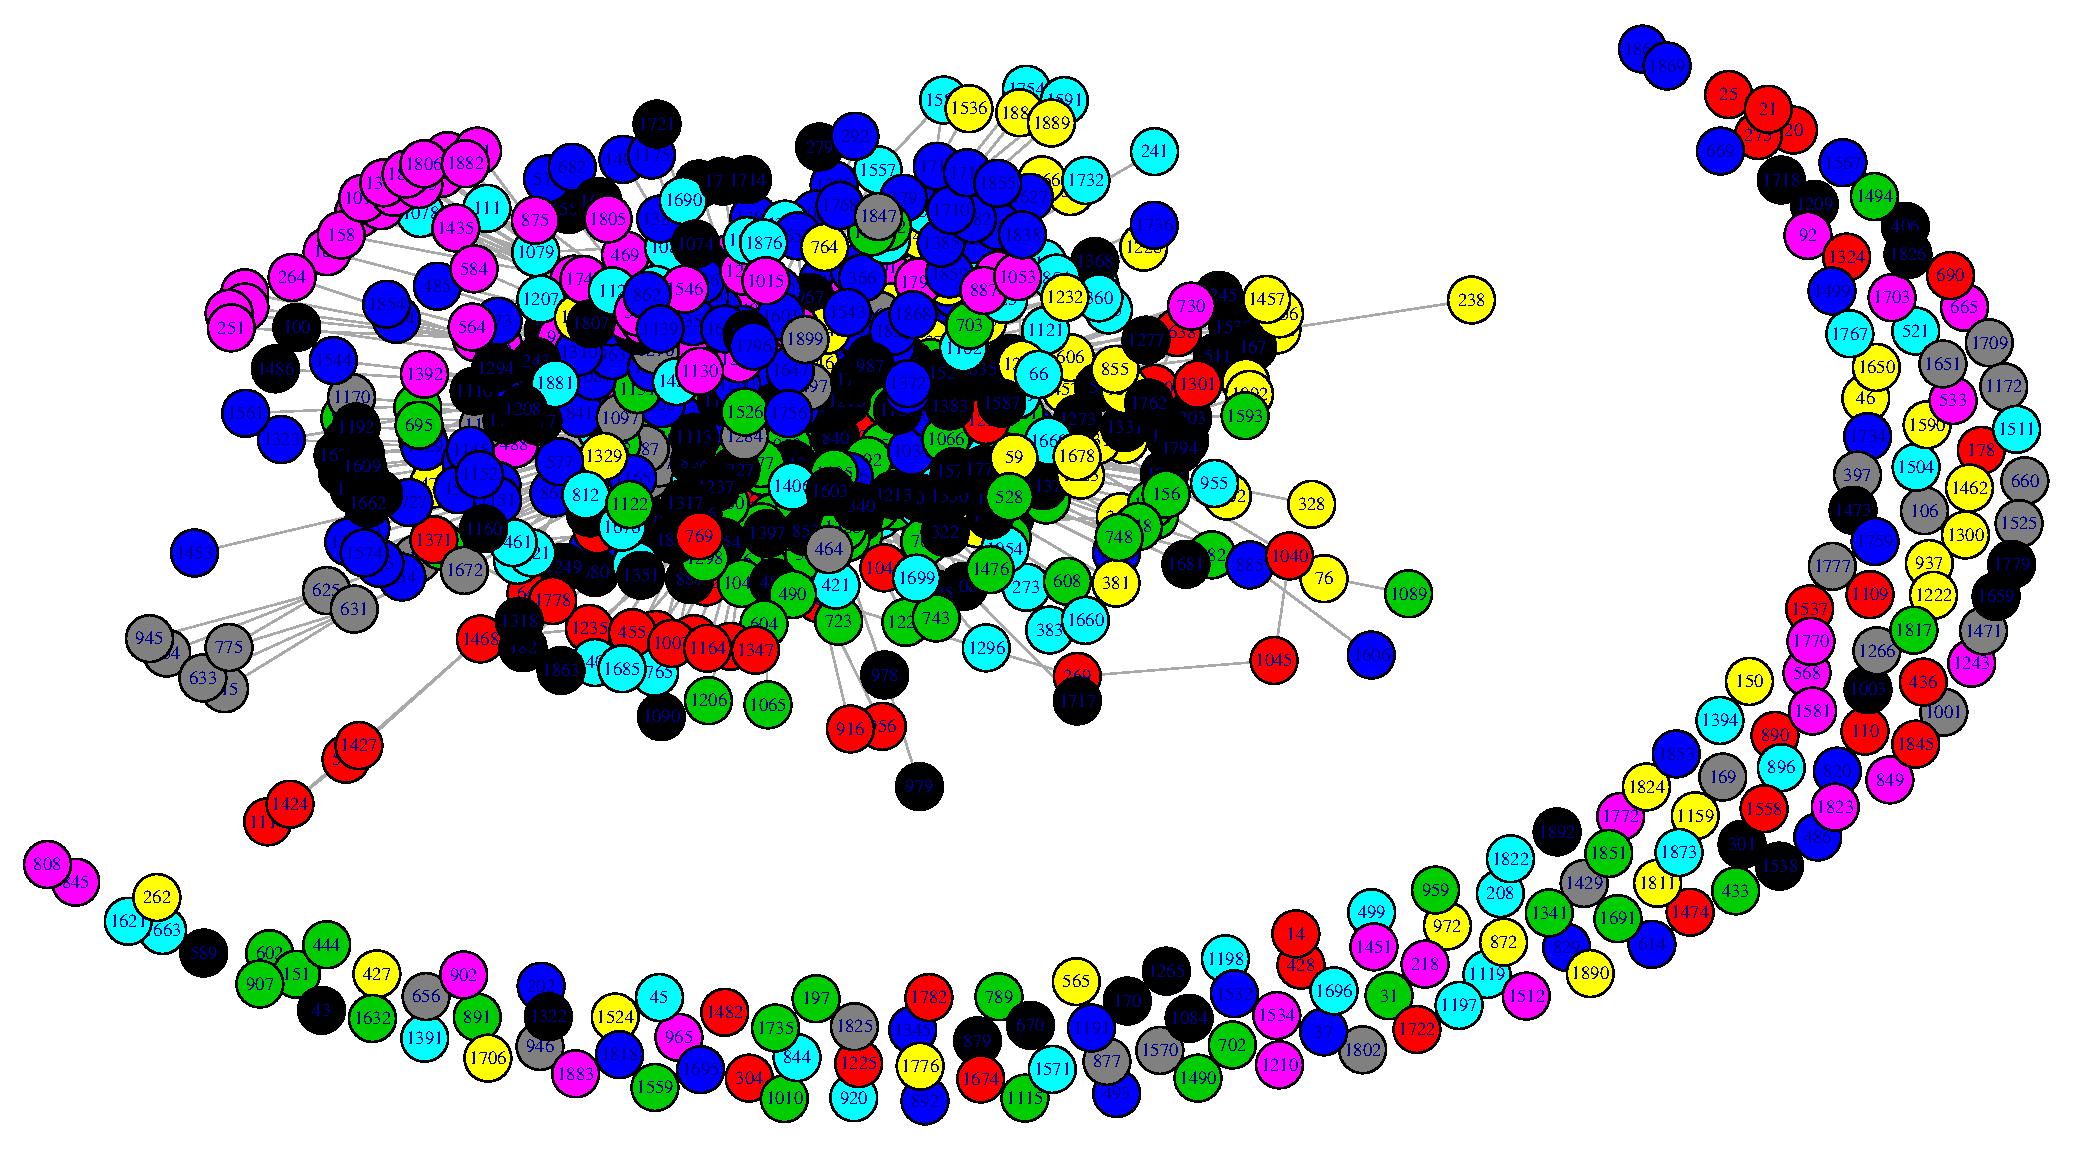
\includegraphics[scale=0.2]{Methods/40percent.eps}
\caption{Clusters with 40\% sampling}
\end{minipage}
\end{figure}
\pagebreak

\begin{figure}[htb]
\centering
\begin{minipage}{0.45\linewidth}
\includegraphics[scale=0.2]{Methods/Cluster_1_.eps}
\caption{Cluster 1}
\end{minipage}
\quad
\begin{minipage}{0.45\linewidth}
\includegraphics[scale=0.2]{Methods/Cluster_2_.eps}
\caption{Cluster 2}
\end{minipage}
\end{figure}
\pagebreak

\begin{figure}[htb]
\centering
\begin{minipage}{0.45\linewidth}
\includegraphics[scale=0.2]{Methods/Screeplot1_.eps}
\caption{Scree Plot 1}
\end{minipage}
\quad
\begin{minipage}{0.45\linewidth}
\includegraphics[scale=0.2]{Methods/Screeplot2_.eps}
\caption{Scree Plot 2}
\end{minipage}
\end{figure}
\pagebreak

\begin{figure}[htb]
\centering
\begin{minipage}{0.45\linewidth}
\includegraphics[scale=0.15]{Methods/AbsCut1_.eps}
\caption{Absolute cut score for cluster 1}
\end{minipage}
\quad
\begin{minipage}{0.45\linewidth}
\includegraphics[scale=0.15]{Methods/AbsCut2_.eps}
\caption{Absolute cut score for cluster 2}
\end{minipage}
\end{figure}

\begin{figure}[htb]
\centering
\begin{minipage}{0.45\linewidth}
\includegraphics[scale=0.15]{Methods/FixCut1_.eps}
\caption{Fixed percentage of population for cluster 1}
\end{minipage}
\quad
\begin{minipage}{0.45\linewidth}
\includegraphics[scale=0.15]{Methods/FixCut2_.eps}
\caption{Fixed percentage of population for cluster 2}
\end{minipage}
\end{figure}
\pagebreak

\begin{figure}[htb]
\centering
\begin{minipage}{0.45\linewidth}
\includegraphics[scale=0.15]{Methods/SdCut1_.eps}
\caption{Standard deviation for cluster 1}
\end{minipage}
\quad
\begin{minipage}{0.45\linewidth}
\includegraphics[scale=0.15]{Methods/SdCut2_.eps}
\caption{Standard deviation for cluster 2}
\end{minipage}
\end{figure}

\begin{figure}[htb]
\centering
\begin{minipage}{0.45\linewidth}
\includegraphics[scale=0.15]{Methods/RandomHist1_.eps}
\caption{Random Permutation Histogram for cluster 1}
\end{minipage}
\quad
\begin{minipage}{0.45\linewidth}
\includegraphics[scale=0.15]{Methods/RandomHist2_.eps}
\caption{Random Permutation Histogram for cluster 2}
\end{minipage}
\end{figure}
\pagebreak

\begin{figure}[htb]
\centering
\begin{minipage}{0.45\linewidth}
\includegraphics[scale=0.15]{Methods/RandomPlot1_.eps}
\caption{Random Permutation for cluster 1}
\end{minipage}
\quad
\begin{minipage}{0.45\linewidth}
\includegraphics[scale=0.15]{Methods/RandomPlot2_.eps}
\caption{Random Permutation for cluster 2}
\end{minipage}
\end{figure}

\subsection{Link Prediction}

\noindent {\bf Problem statement:} To apply efficient link prediction algorithms to uncover developer
relations and to predict future outcomes.

\noindent {\bf Dataset Used:}
\begin{enumerate}
\item {\em Co-authorship data}: This dataset contains authors where they are represented by the unique author's ID's.
A relation exists between two author ID's only if both have coauthored a book. Each author can be involved
in writing more than one book. In the graph format authors are represented by nodes or vertices and the
relations between them are represented by the presence of edge between them.
This is an undirected graph having 757 vertices and 1000 edges. 

\item {\em Email Communication Data}: This dataset contains the IDs of individuals who are actively involved
in a communication network via email. A relation between two IDs exist if any one of the two individuals
communicate through email. In the graph format, individuals are represented by nodes or vertices and the
relations between them are represented by the presence of edge between them. This is a directed graph having 1133 vertices and 10903 edges.
\end{enumerate}

\noindent {\bf Pseudocode/Algorithm}

\noindent Data : Weighted RawDataFrame\\
\noindent Result : Edges with corresponding similarity scores

\begin{itemize}
\item Step 1 : Convert the data frame into graphs . Directed or undirected based on the data.
\item Step 2 : Remove all self loops and repeated edges.
\item Step 3: Compute probabilities of existence and non-existence of any link in the graph
\item Step 4: Compute clusters using fast greedy approach
\item Step 5: Given a non existent link,
\begin{itemize}
\item a) Compute total number of common neighbours
\item b) Compute number of common neighbours within common groups
\item c) Determine from a) and b) the number of common neighbours outside of common groups
\end{itemize}
\item Step 6: Compute the similarity score
\item Step 7: Sort all the edges in the decreasing order of their similarity scores
\end{itemize}

\noindent {\bf Procedure}

Given a weighted social network dataset, link prediction can be performed by using the structural properties
of the network and community information of the nodes present in the network. This process is performed using
R software which is a data mining tool for Big data. R packages such as igraph, sna, proxy are used. A feature
rich, weighted social network dataset is taken as the input. It is converted into graph with no self loops and
repeated edges. To obtain community information of the nodes in the graph, a fast greedy algorithm is applied.
The probabilities of existence and non-existence of any link in the graph is computed. Now, given any non-existent link,
the number of common neighbours within and outside of common groups and the total number of common neighbours is computed.
Using the parameters computed above a similarity score is assigned to every non-existent link. All the links are sorted
in the decreasing order of their similarity score.

\noindent {\bf Results}

Results of the analysis are shown in Table 4.5.

\begin{table}[htb]
\centering
\begin{tabular}{ccl}\hline
from & to & probability\\ \hline
11 & 14 & 0.07272727\\
11 & 15 & 0.07272727\\
14 & 11 & 0.07272727\\
14 & 15 & 0.07272727\\
15 & 11 & 0.07272727\\
15 & 14 & 0.07272727\\
11 & 13 & 0.04848485\\
11 & 44 & 0.04848485\\
11 & 66 & 0.04848485\\
13 & 11 & 0.04848485\\
\vdots&\vdots&\vdots\\ \hline
\end{tabular}\label{Table2}
\caption{Probabilities for edges}
\end{table}


\subsection{Time Series Analysis}

\noindent {\bf Problem statement:}
Time Series Analysis provides us with a pragmatic view of the overall network with respect to time in a
dynamic fashion in order to understand the growth, evolution and the final outcome of the social network
by the effective use of time varying graphs and temporal indicator metrics.

\noindent {\bf Dataset Used:}
\begin{enumerate}
\item {\em Twitter data}: This dataset contains where twitter-user's the they are represented by the unique
twitter ID's. A relation exist between two twitter ID's only if both have had an interaction. The twitter
users having one or many interactions at any given time. In the graph theory paradigm twitter users are
represented by nodes or vertices and time used as a sole parameter to evaluate them.

\item {\em Source-Forge data}: This is a dataset which contains unique developer ID's and their interactions over time.
In the graph theory paradigm developers are represented by nodes or vertices and time used as a sole parameter to evaluate them.
\end{enumerate}

\noindent {\bf Pseudocode/Algorithm}

\noindent Result : Complete analysis and growth of the network over time.

\begin{itemize}
\item Step 1 : Load dataset with nodes, edges and time stamps.
\item Step 2 : Generate an initial sub-graph with a suitable colour pallete.
\item Step 3 : Generate subsequent layout using graphopt with normalized coordinates.
\item Step 4 : Determine a suitable time slot and generate other subgraphs illustrating growth.
\item Step 5 : Time loop starts and remove edges which are not present.
\item Step 6 : A final graph is obtained indicating all the interactions.
\item Step 7 : The most influential person in the network is determined.
\end{itemize}

\noindent {\bf Procedure}

A suitable twitter dataset has been analysed dynamically in order to understand the growth of the social network.
Temporal graph and time varying graph algorithms are rigorously implemented. It is of interest to understand the evolution
of the network and forecast the most influential entity. Snapshots of the subnetworks are generated periodically.
The final network shows interactions of all the individuals in the network. The following snapshots are clubbed into
flash content in order to get aesthetically stimulating result.

\noindent {\bf Results}

Results of the analysis are shown in Table 4.6 and Figures 4.19 - 4.21.

\begin{table}
\centering
\begin{tabular}{lll}\\ \hline
\multicolumn{3}{c}{Input}\\ \hline
id1 & id2 & time \\ \hline
1 & 2 & 1 \\
1 & 3 & 1 \\
2 & 3 & 1 \\
5 & 3 & 2 \\
6 & 2 & 3 \\
7 & 2 & 4 \\
8 & 7 & 5 \\
9 & 5 & 6 \\
10 & 7 & 7 \\
\vdots & \vdots &\vdots\\ \hline
\end{tabular}
\caption{Time Series Analysis of Twitter Data}
\end{table}

\begin{figure}[hb]
\centering
\begin{minipage}{0.45\linewidth}
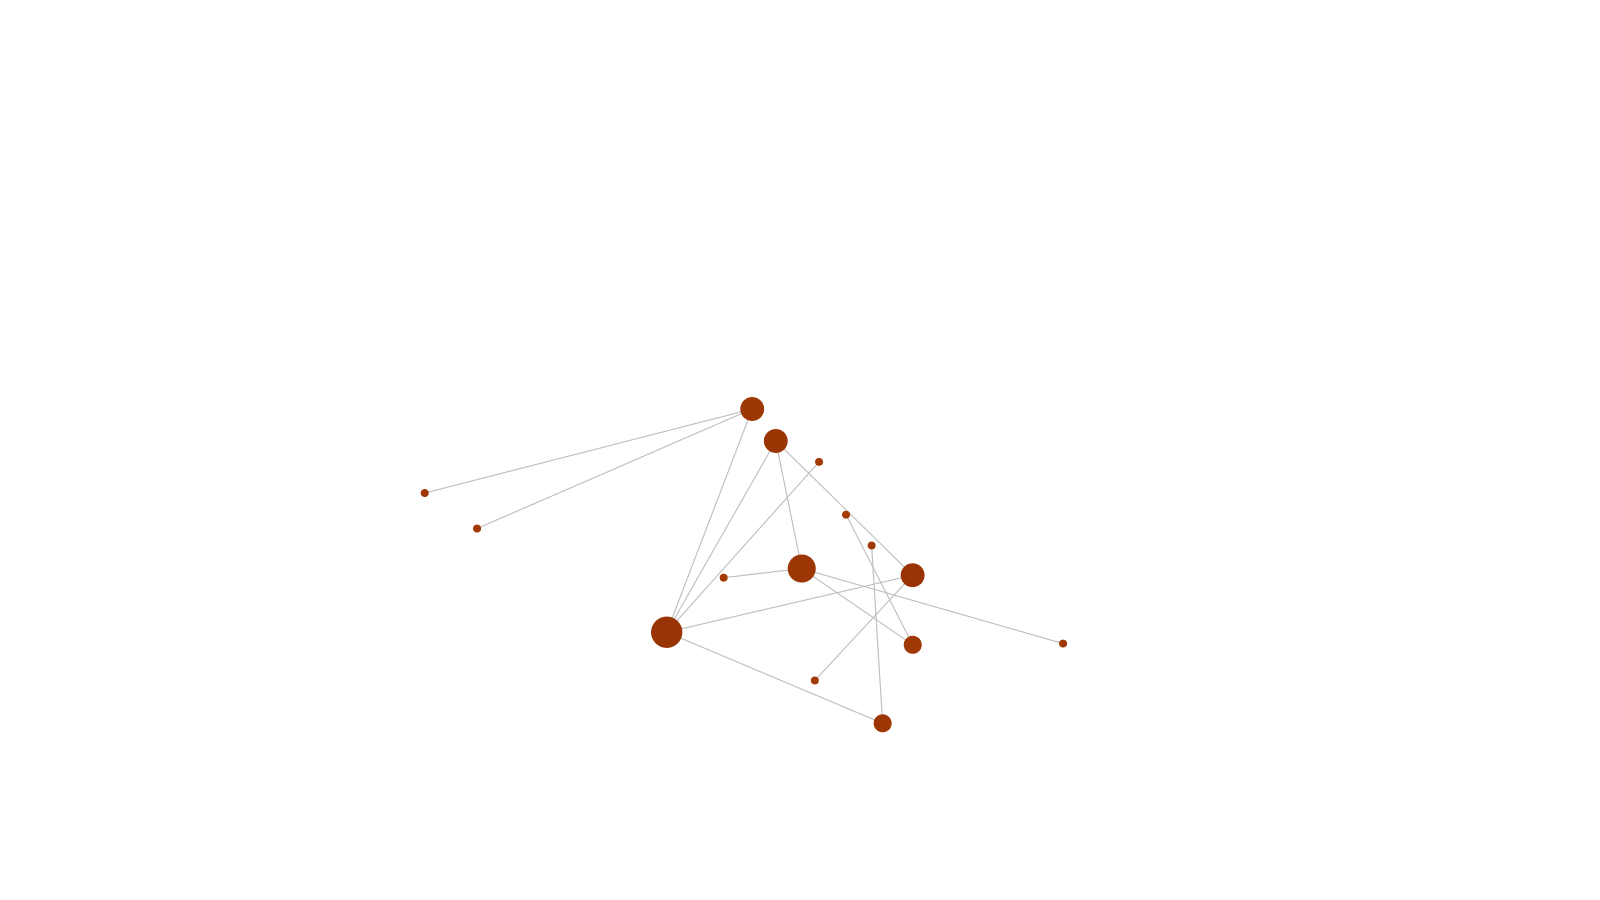
\includegraphics[scale=0.15]{Methods/example104.eps}
\caption{At first time instance}
\end{minipage}
\quad
\begin{minipage}{0.45\linewidth}
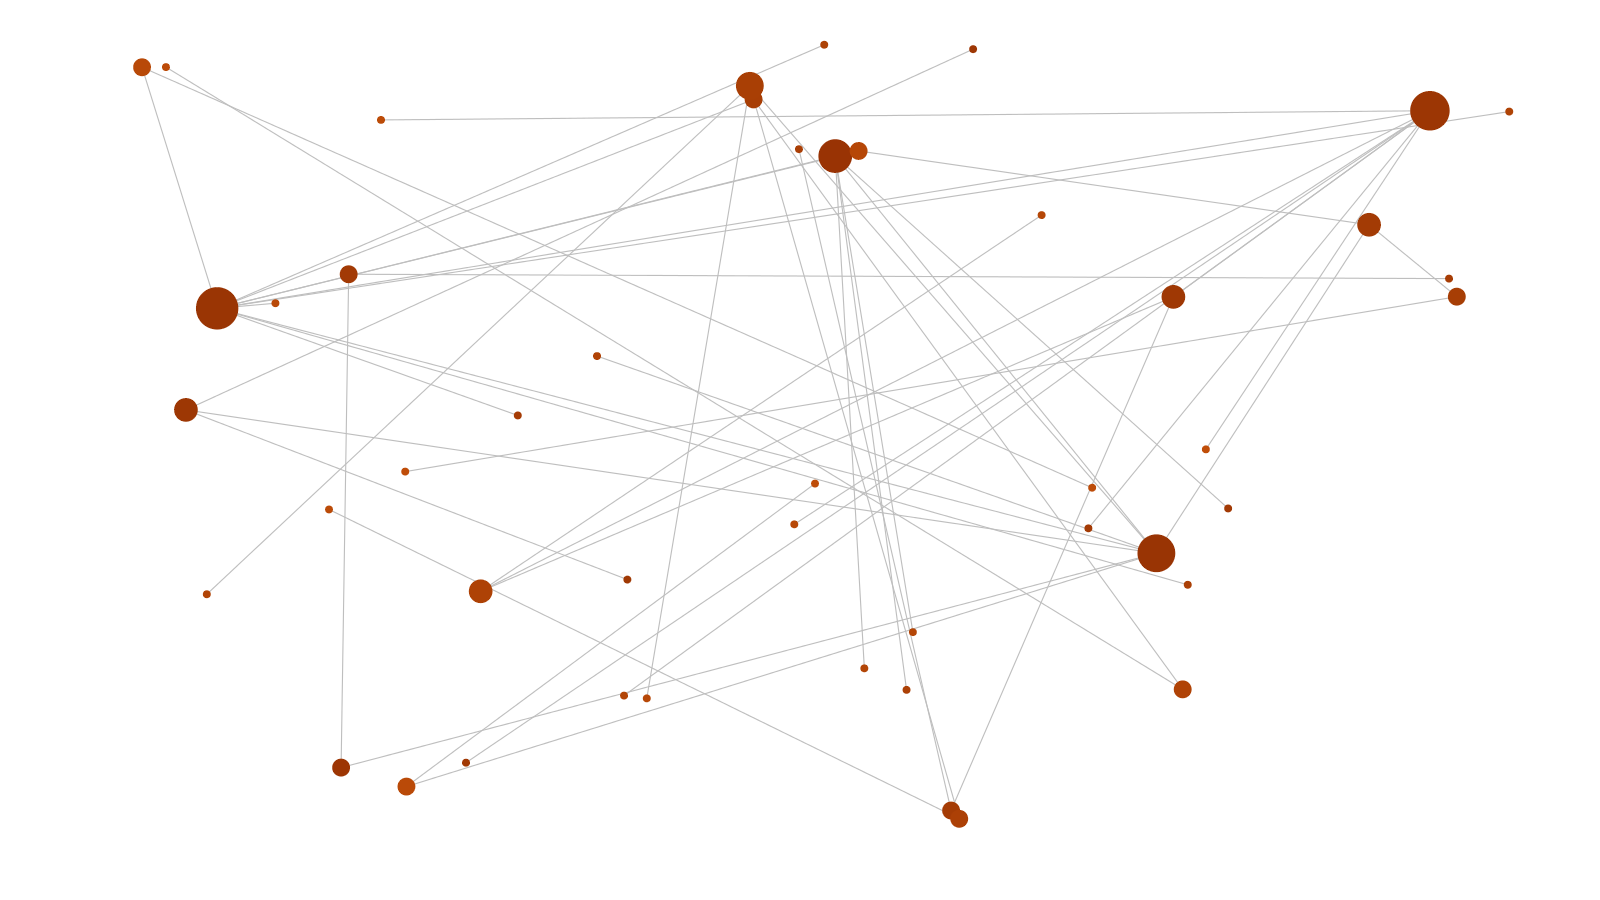
\includegraphics[scale=0.15]{Methods/example425.eps}
\caption{At second time instance}
\end{minipage}
\end{figure}
\begin{figure}
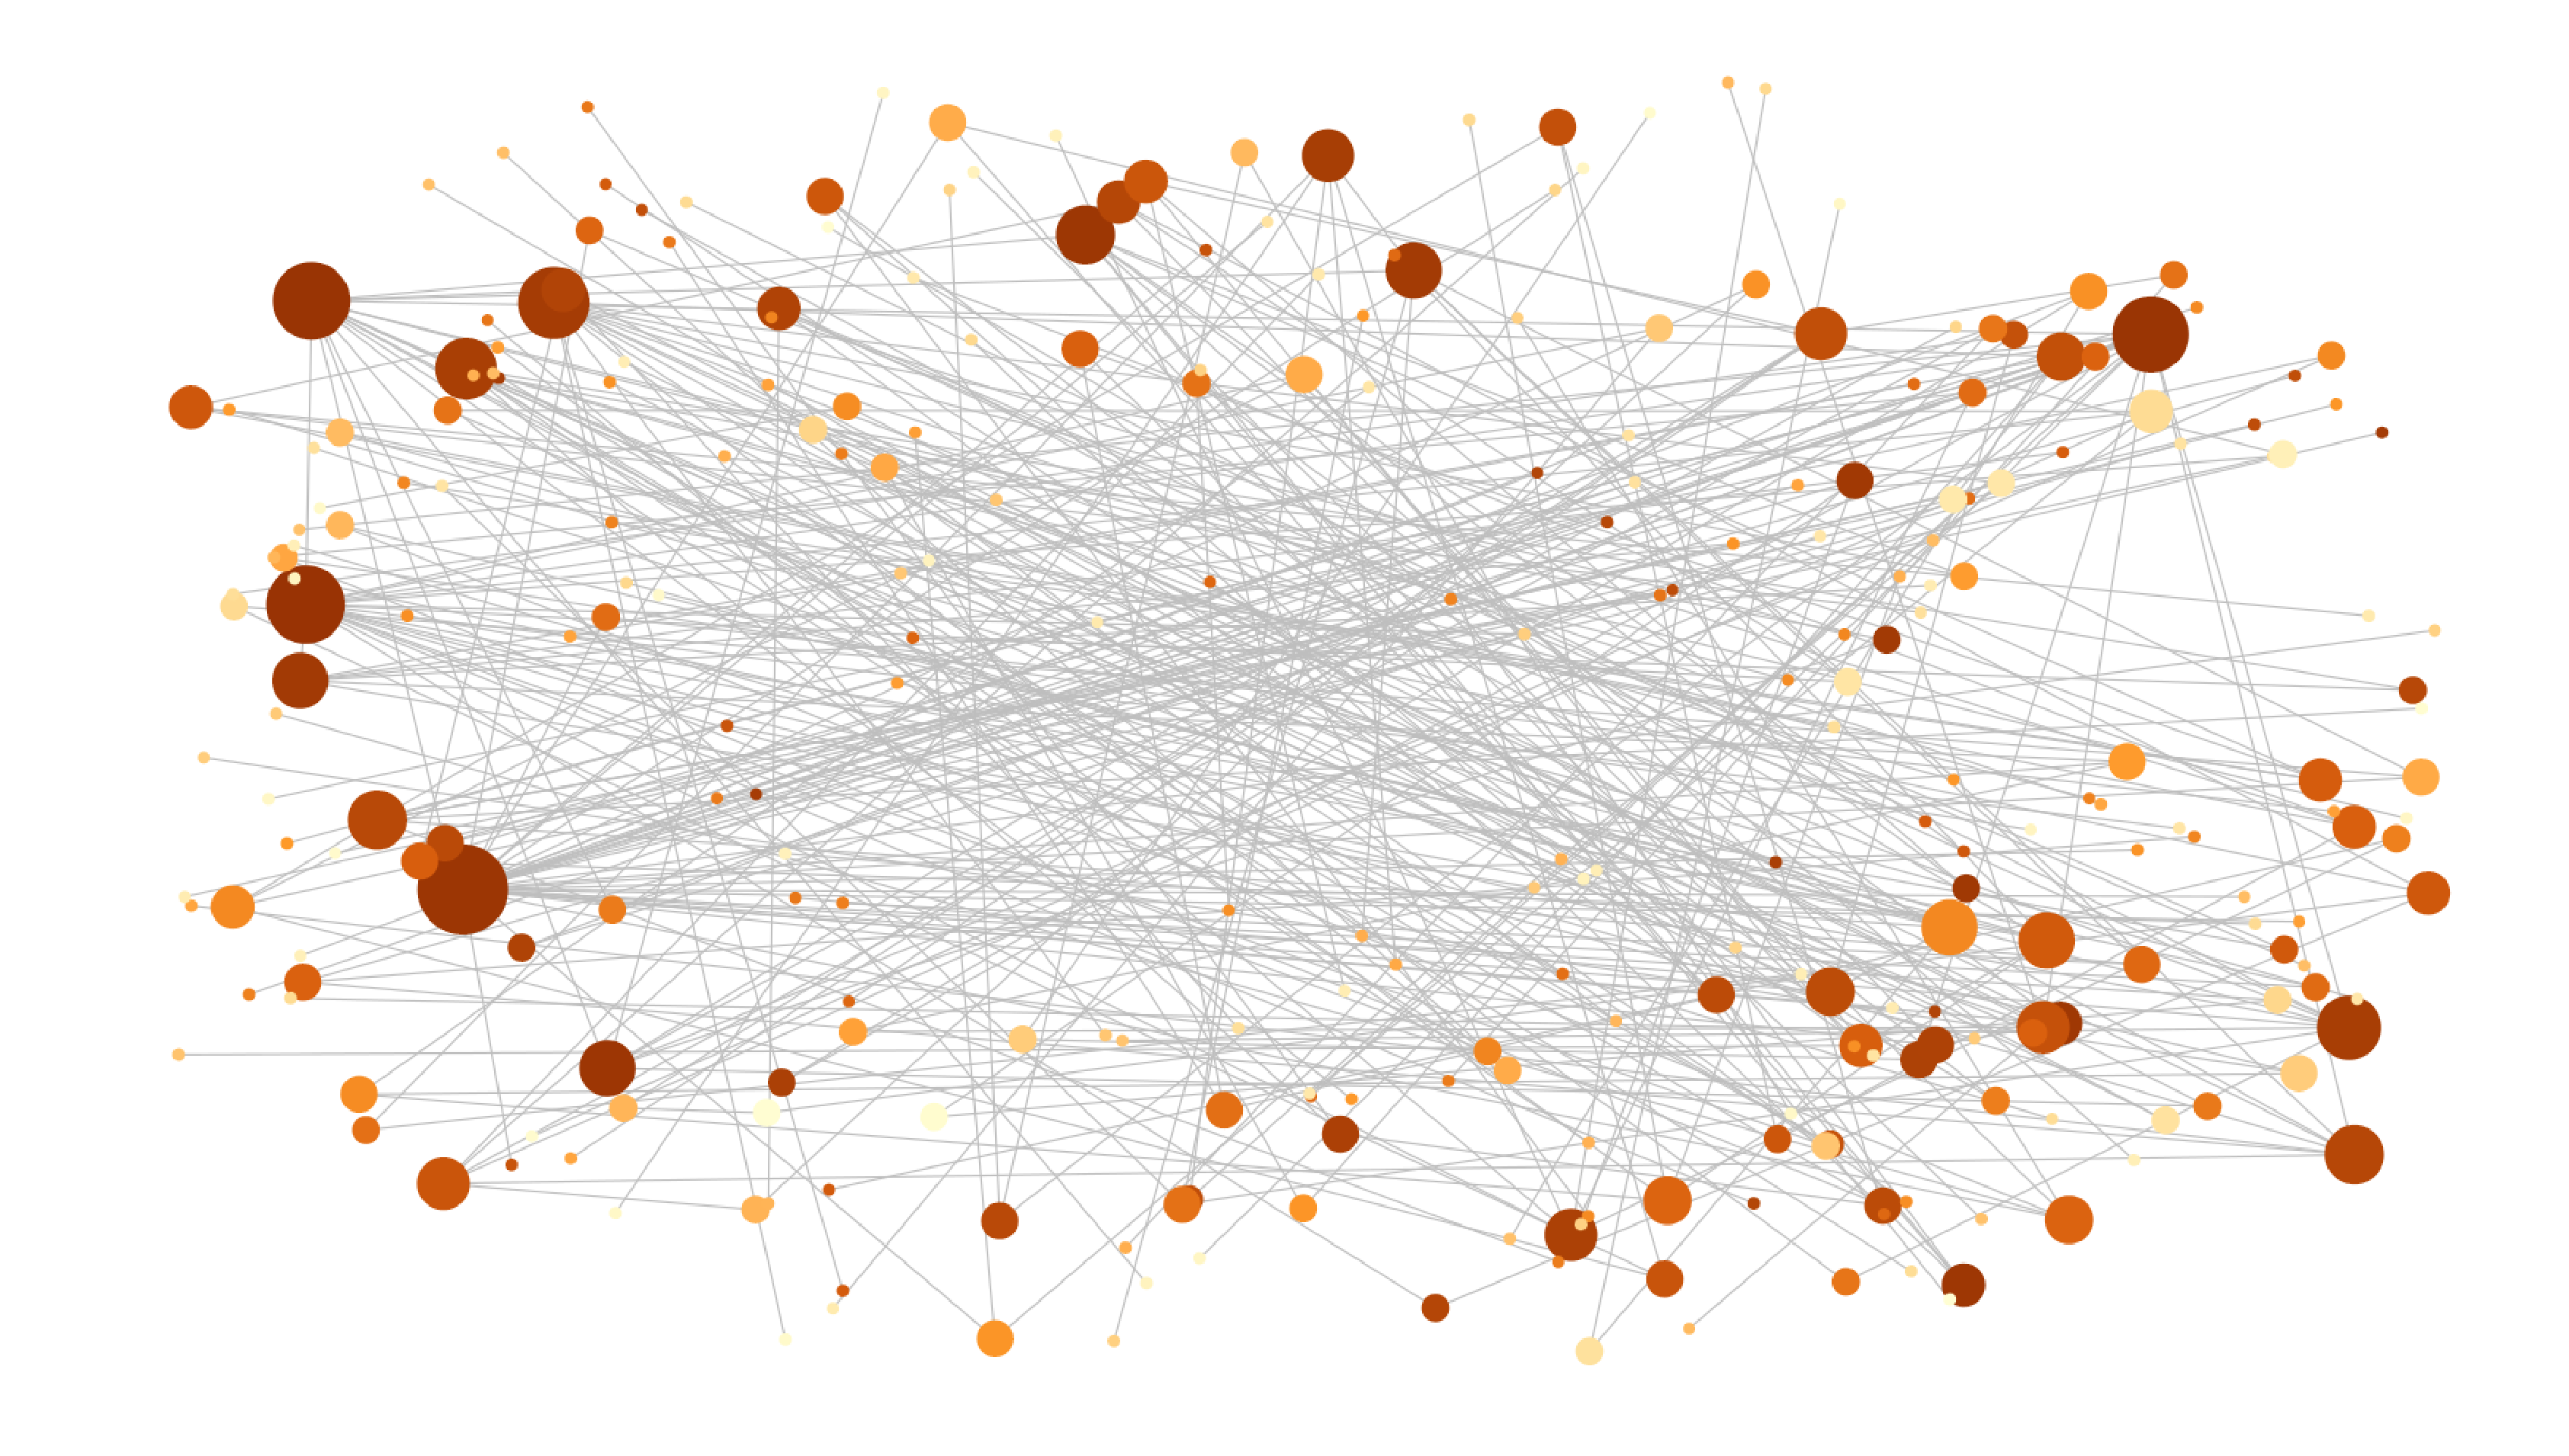
\includegraphics[scale=0.3]{Methods/example2971.eps}
\caption{At the final time instance}
\end{figure}

% ------------------------------------------------------------------------


%%% Local Variables:
%%% mode: latex
%%% TeX-master: "../thesis"
%%% End:

